\subsection{Timing Performance Results from Calorimeter with SiPM Readout}
\label{sec:beamtiming}

As the time measurement precision depends on the rise time of the pulse we first
measure the rise time for signals observed in the calorimeter cell. The rise
time of these signals are driven by the time constants of the wave length
shifter as we demonstrated in reference~\cite{lysotiming}. In figure
\ref{RiseTime} we show the rise time of the pulses as a function of the signal
amplitude. We observe that the the rise time of the pulses becomes shorter for larger pulses, 
reaching around 2 ns for the largest amplitudes in each channel. 
The amplitude dependency of the rise time is similar between different types of SiPMs but 
reaches its shortest value at different signal amplitudes. 

%
\begin{figure}[htb]
%\hspace*{-0.3cm}
%\begin{minipage}[b]{22pc}
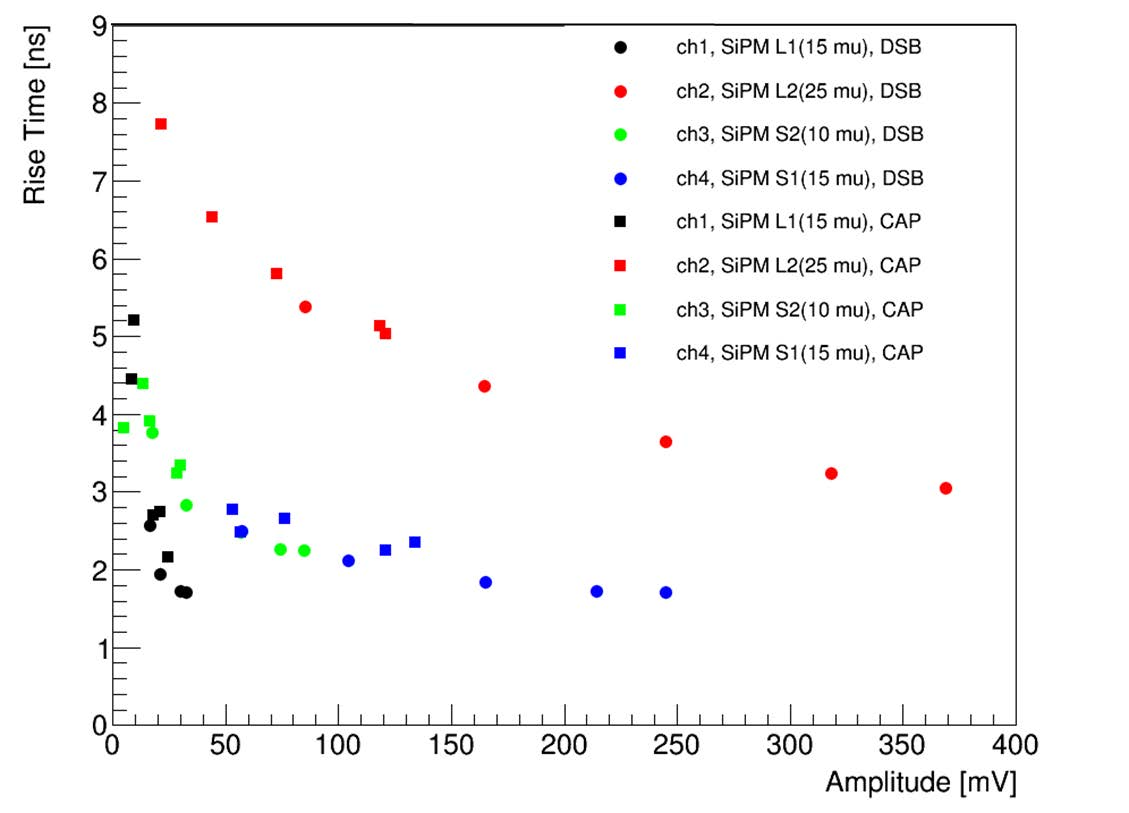
\includegraphics[width=0.99\textwidth]{RiseTime.pdf}
%\end{minipage}
%\begin{minipage}[b]{14pc}
\caption{\label{RiseTime}Rise time of the pulses as a function of the amplitude
for the four different SiPMs. The data recorded with the plastic fibers and the
quartz capillaries are distinguished as dots and squares. For each of the two
data sets with plastic fibers and capillaries there are 5 measurements
corresponding to beam energies of 20, 50, 100, 150 and 200 GeV.}
%\end{minipage}
%\hspace*{-0.3cm}
\end{figure}
%

In figure \ref{TimeResolution} we show the time resolution of the four
individual fibers as a function of their respective signal amplitude. We observe 
that the time resolution improves as the amplitude of the pulses increases, 
similar to the behavior for the rise time. However, the resulting improvement in 
signal to noise results in additional improvement beyond just the improvement due
to faster rise time. 

%
\begin{figure}[htb]
%\hspace*{-0.3cm}
%\begin{minipage}[b]{22pc}
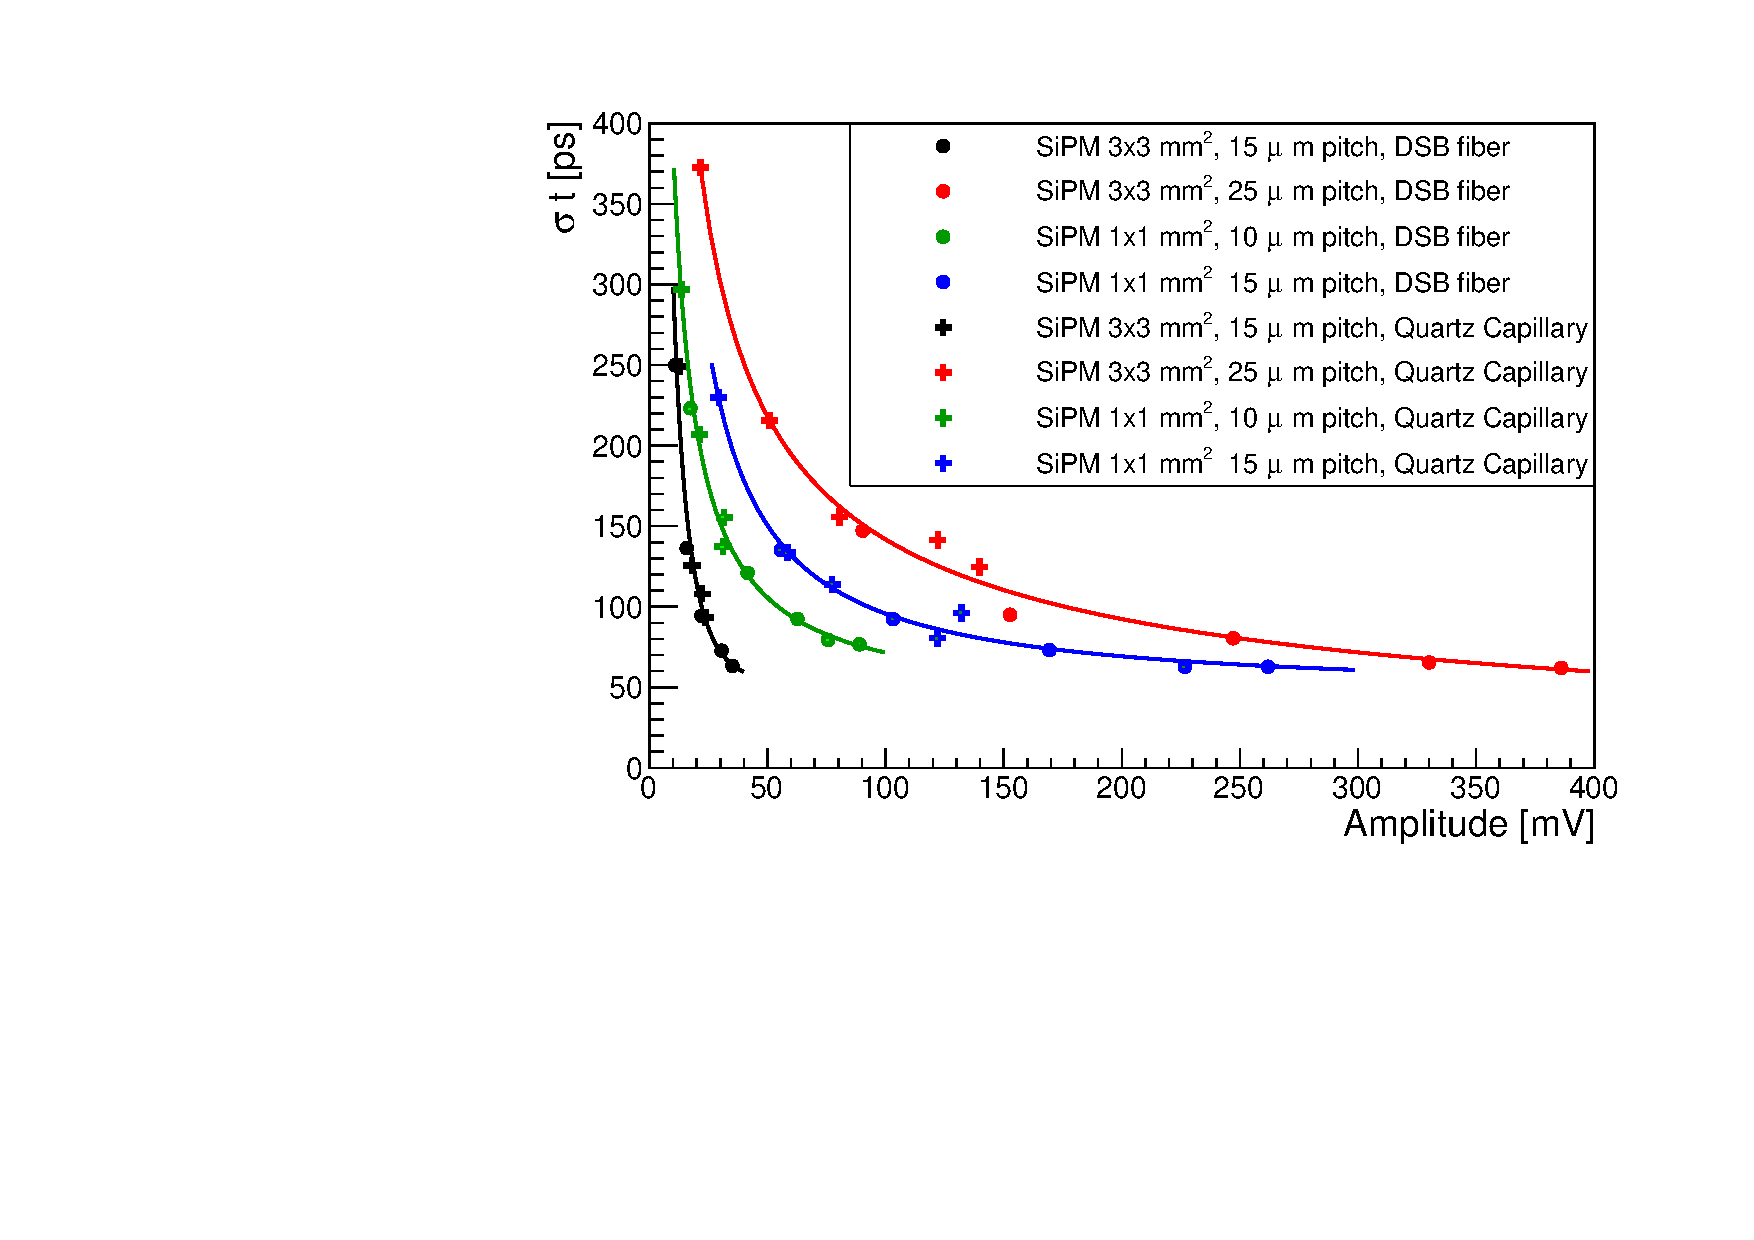
\includegraphics[width=0.99\textwidth]{figures/ShashlikTimeResolution.pdf}
%\end{minipage}
%\begin{minipage}[b]{14pc}
\caption{\label{TimeResolution} Time resolution achieved with the calorimeter cell using the signal of each 
of the  SiPMs individually. The data for each SiPM consists of two sets, one with the DSB WLS plastic fiber and one with 
the capillaries with a liquid DSB based WLS. The time resolution improves with increasing signal amplitude. The best time 
resolution per fibre is around $60$~ps for all of the channels. The amplitude at which this performance is achieved varies.}
%\end{minipage}
%\hspace*{-0.3cm}
\end{figure}
%


For the same amplitude we find the same timing resolution with the capillaries
and the plastic WLS fibers, both using DSB WLS agent. This further supports our
previous findings that the the light propagation in the optical elements of a
scintillation based calorimeter does not significantly affect the performance at
the level of $50$~ps.

The light extraction efficiency of capillaries with liquid WLS remains
sufficiently high for dose rates of $100$~Mrad and beyond and for fluences of
$10^{14}$~protons/$\mathrm{cm}^{2}$ and beyond~\cite{shashlik2}. The
energy resolution performance of the LYSO-tungsten cell is not limited by
photo-statistics but is rather limited by the sampling fraction. The timing
performance at lower energies could be improved by increasing the raw signal.
This could be achieved by using larger diameter capillaries.\\ 

